\begin{figure}[ht] %s state preferences regarding figure placement here

% use to correct figure counter if necessary
%\renewcommand{\thefigure}{2}

\centering
\subfigure[Physical specimen collection]{%
\label{fig:collection-a}%
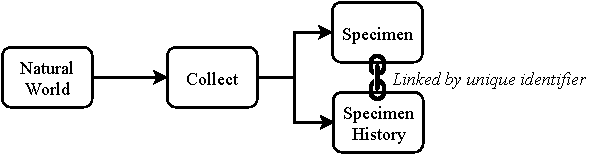
\includegraphics[scale=1]{figures-fig1a.pdf}} \\
\subfigure[Digital data collection]{%
\label{fig:collection-b}%
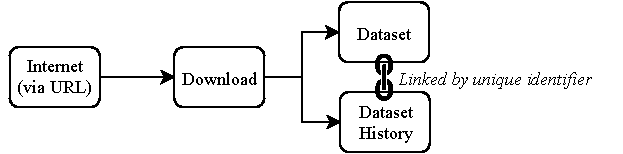
\includegraphics[scale=1]{figures-fig1b.pdf}}%

\caption{Reliable record keeping for digital datasets \subref{fig:collection-b} can be achieved in an analogous way to current practices in record keeping for physical specimens \subref{fig:collection-a}. Biologists collect physical specimens from the natural world, thoroughly document the process, then store the specimens in facilities equipped for long-term preservation. Analogously, digital datasets that are downloaded from the internet can be thoroughly documented and archived in dedicated repositories for long-term preservation. Just as the collection of physical specimens is recorded and identified in specimen information records, the downloading of digital datasets can also be recorded and identified in dataset provenance records.}%

\label{fig:collection} % \label works only AFTER \caption within figure environment

\end{figure}

